\chapter{前言}
\renewcommand{\baselinestretch}{10.0} %設定行距
\pagenumbering{arabic} %設定頁號阿拉伯數字
\setcounter{page}{1}  %設定頁數
\fontsize{14pt}{2.5pt}\sectionef
\section{檔案說明}
%=--------------------檔案說明----------------------=%
共經歷了八個版本改版\\
前七個版本:
\href{https://mdecd2023.github.io/football-apj1/downloads/ag4/bubbleRob%E7%B4%80%E9%8C%84.7z}{bubbleRob紀錄.7z}\\
最終版:
\href{https://mdecd2023.github.io/football-apj1/downloads/ag4/bubbleRob.7z}{bubbleRob.7z}\\
裡面包含了\\
\\
\begin{figure}[hbt!]
\begin{center}
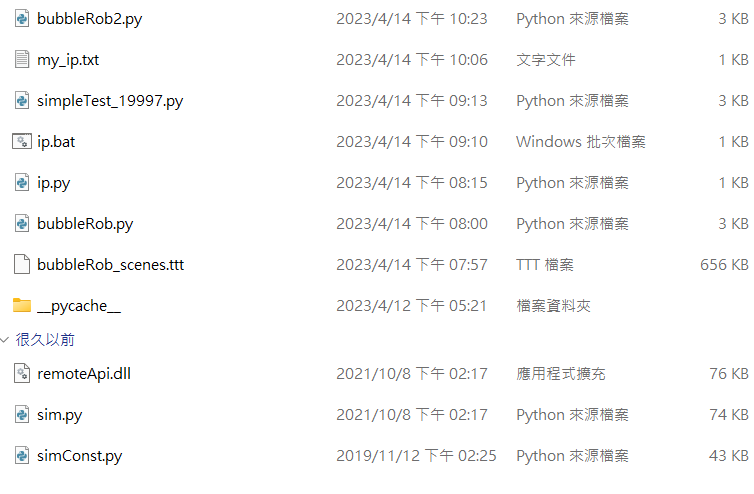
\includegraphics[width=16cm]{遊戲檔案}
\caption{\Large 遊戲檔案}\label{遊戲檔案}
\end{center}
\end{figure} 
\qquad \\
點擊ip.bat就能直接獲取到目前電腦的ipv4位置\\
\begin{figure}[hbt!]
\begin{center}
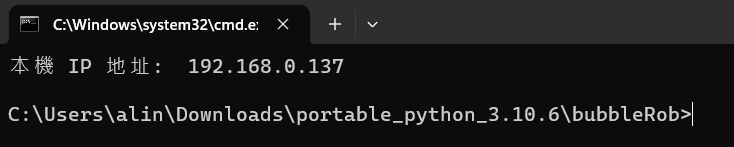
\includegraphics[width=16cm]{ip}
\caption{\Large 目前電腦ip}\label{目前電腦ip}
\end{center}
\end{figure} 
\qquad \\
\\
\\
\\
 加入遊戲所在電腦ip 只需輸入ip (遊戲所在電腦ip)
 \begin{figure}[hbt!]
\begin{center}
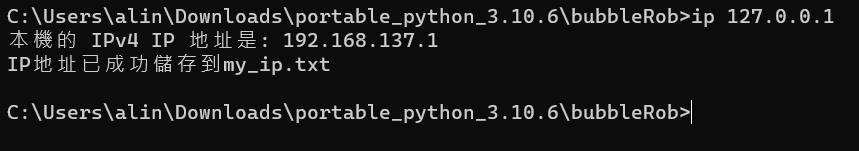
\includegraphics[width=16cm]{gameip}
\caption{\Large gameip}\label{gameip}
\end{center}
\end{figure} 
\section{遊戲說明}
%=--------------------遊戲說明----------------------=%
開啟場景後便可以使用19997進行連線,
如果成功連線便會顯示\\
welcome to play\\
\begin{figure}[hbt!]
\begin{center}
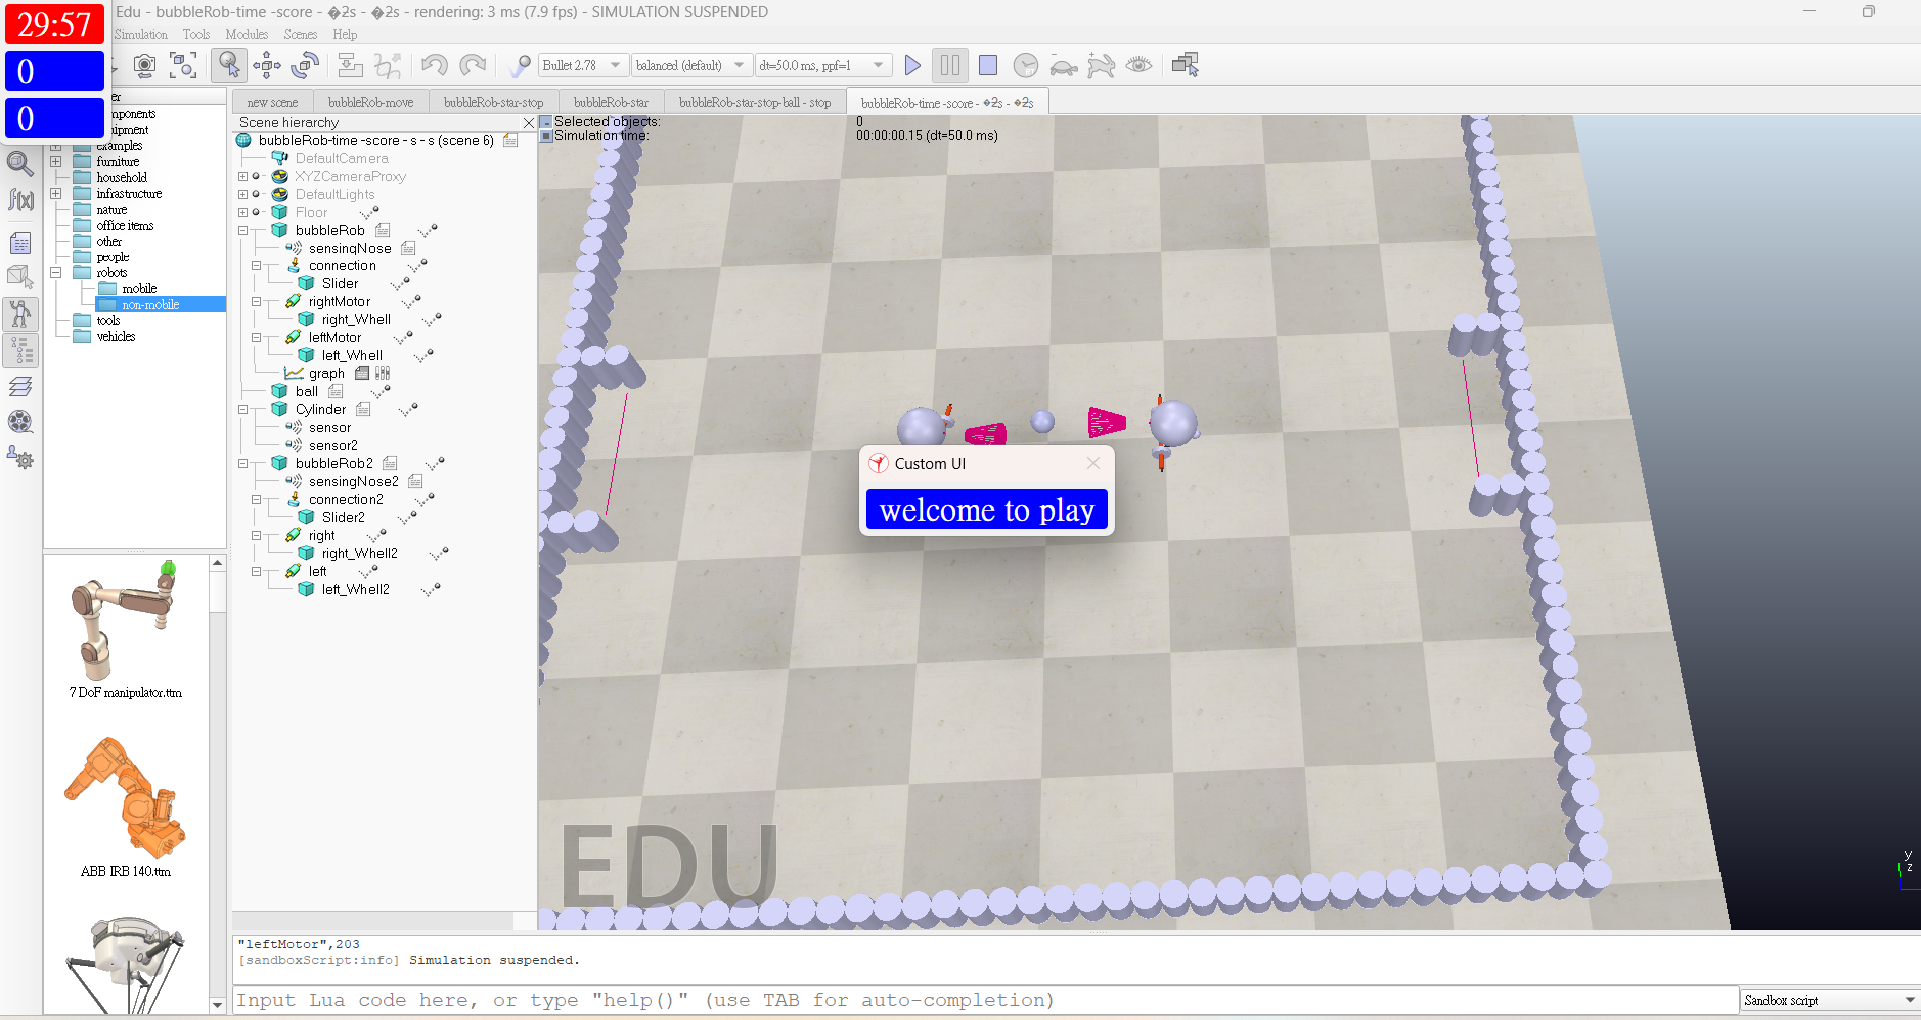
\includegraphics[width=14cm]{412-1}
\caption{\Large 歡迎}\label{歡迎}
\end{center}
\end{figure} 
\qquad \\
這時23020與19998埠號便會開啟,
第二位玩家便可利用19998加入遊戲,
加入成功便會立即開始,
觀戰者可以利用23020埠號進行觀戰
\section{規則說明}
%=--------------------規則說明----------------------=%
 遊戲規則簡單,透過操控bubbleRob將球打入對方球門即得一分,時間內其中一方分數高獲勝。\\
遊戲規則如下:
\begin{enumerate}
\item 利用wasd操控移動方向。
\item 將球打入敵方球框即得一分。
\item 一方得分後便會暫停遊戲並還原場地。
\item 按下p則繼續遊戲。
\item 時間內進球數多的一方獲勝。
\item 時間到即停止遊戲。
\end{enumerate}

\renewcommand{\baselinestretch}{0.5} %設定行距